\documentclass[twocolumn,tighten,longauthor]{myaastex62}
%\documentclass[twocolumn,tighten,longauthor,trackchanges]{myaastex62}
\bibliographystyle{bibstyle}
\shorttitle{An optimized algorithm to search for transits of small extrasolar planets}
\shortauthors{Hippke \& Heller}
\newcommand\RH[1]{\textcolor{red}{\bf #1}}
\usepackage{amsmath}
\begin{document}
\title{Transit Least Squares: An optimized algorithm to search for transits of small extrasolar planets in stellar light curves from Kepler, TESS, and PLATO}

\author[0000-0002-0794-6339]{Michael Hippke}
\affiliation{Sonneberg Observatory, Sternwartestr. 32, 96515 Sonneberg, Germany}
\email{michael@hippke.org}

\author[0000-0002-9831-0984]{Ren\'{e} Heller}
\affiliation{Max Planck Institute for Solar System Research, Justus-von-Liebig-Weg 3, 37077 G\"ottingen, Germany}
\email{heller@mps.mpg.de}


\begin{abstract}
We present a new method to detect planetary transits from time-series photometry. While the commonly used Box-Least-Squares (BLS) algorithm searches for rectangular signals, we fit for transit-like limb-darkened shapes. Compared to BLS, our method yields a 5--10\,\% higher detection efficiency at the same false alarm rate. This comes at the cost of higher computational load ($\sim100\,$x). A single Kepler K2 light curve can be searched optimally in 5\,min on a laptop computer (BLS: 15\,s), and in X\,s using a consumer-grade graphics card. The \texttt{Transit Least Squares} package is open source and publicly available at \url{github.com/hippke/tls}.\\
\end{abstract}


\section{Introduction}
The first detection of a planetary transit  was made after radial velocity variations indicated the presence of a Jupiter-mass body orbiting HD 209458 \citep{2000ApJ...529L..45C}. Observations near the predicted transit time showed a highly significant dip in brightness and confirmed the presence of the planet. Subsequent searches focused on individual stars with known planets and known expected transit times \citep{2005ApJ...633..465S,2005A&A...444L..15B}, where the screening for transits could be done by-eye, because the stars were bright and the planets big, causing deep transits with high signal-to-noise ratios (SNR). 

Exoplanet surveys have since expanded greatly in numbers and volume. Ground-based mass surveys such as HATNet \citep{2004PASP..116..266B}, WASP \citep{2006PASP..118.1407P}, KELT \citep{2007PASP..119..923P}), and CHESPA \citep{2018arXiv180901789Z}, and space-based search campaigns like CoRoT \citep{2009A&A...506..411A}, Kepler \citep{2010Sci...327..977B}, K2 \citep{2014PASP..126..398H}), and TESS \citep{2014SPIE.9143E..20R} produce vast dataset. These encompass hundreds of thousands of stars, cadences of seconds or minutes, and observational duty cycles that span several years. These modern exoplanet transit searches require fast, reliable and sensitive algorithms to detect the expected but unknown transit signals.

The Box Least Squares (BLS) algorithm \citep{2002A&A...391..369K,2016ascl.soft07008K} has become the standard tool for exoplanet transit searches in large data sets. It approximates the transit light curve as a (negative) boxcar function with a normalized average flux of zero (out of transit) and a fixed depth during the transit. This approach is key to its computational speed, and allows for a reliable detection of high to medium SNR signals, such as large and moderately large planets, e.g. for Jupiter- or Neptune-sized planets around sun-like stars in most surveys. For lower SNR signals, such as the particularly interesting Earth-sized planets orbiting sun-like stars, its detection efficiency decreases dramatically. While this is partly caused by instrumental and stellar noise, an additional component of noise comes from the mathematical concept of the boxcar function. It is equivalent to the astrophysical assumption of no stellar limb darkening and it neglects the effects of the planetary ingress and egress on the transit shape in the light curve. These approximations introduce an extra noise component in the test statistic, thereby diluting the signal. Our new method removes most this noise and thus allows for a better sensitivity.

The BLS algorithm has been analyzed and optimized in depth, e.g. in terms of the optimal frequency sampling \citep{2014A&A...561A.138O}, and it has been extended to variable intervals between successive transits \citep{2013ApJ...765..132C}, to work with non-Gaussian errors \citep{2014IAUS..293..410B}, to improve speed at the cost of sensitivity \citep{2008A&A...492..617R}, and to refine the detected transit parameters \citep{2006MNRAS.373..799C}. Further adaptions were made for the application to circumbinary planets \citep{2008MNRAS.387.1597O}.

Alternative algorithms to BLS exist, but are less popular. The ``matched filter'' algorithm is similar to BLS and also models the transit as a boxcar, but it uses a different test statistic \citep{1996Icar..119..244J,2007ASPC..366..145B}. Phase dispersion minimization \citep{1978ApJ...224..953S} has been shown to be inferior to BLS for transit detection \citep{2002A&A...391..369K}. Analysis of variance (AoV) \citep{2006MNRAS.365..165S} also uses a box-shaped transit model (which the authors refer to as top-hat), and has been demonstrated to have a lower detection efficiency than BLS in WASP data \citep{2012A&A...548A..48E}. Bayesian algorithms can search for any signal form \citep{2000ApJ...535..338D,2001A&A...365..330D}, but are not widely used. For example, the Gregory-Loredo method for Bayesian periodic signal detection uses step-functions (boxes with multiple steps) \citep{2002A&A...395..625A,2004MNRAS.350..331A}. Wavelet-based algorithms \citep{2007A&A...467.1345R} are of similar detection efficiency but have not been widely used except for a dedicated analysis of CoRoT data \citep{2009IAUS..253..374R}. Although polynomials have been suggested to approximate transit shapes more adequately than boxes \citep{2012A&A...548A..44C}, this idea has only been used occassionally \citep{2016AJ....151..171J,2018AJ....156...78L} and without any comparison to BLS in terms of detection efficiency and computational effort.

Comparison of different algorithms showed that BLS is the best of all known algorithms for weak signals \citep{2003A&A...403..329T,2003A&A...408L...5T}, but ``no detector is clearly superior for all transit signal energies'', which has been verified by empirical tests of the methods \citep{2005A&A...437..355M}.

New techniques have now arrived with the advent of artificial intelligence. Deep learning algorithms are usually trained with a series of transit shapes  \citep{2018MNRAS.474..478P,2018AJ....155..147Z,2018MNRAS.478.4225A}. Random-Forest methods detect 7.5\,\% more planets than classical BLS for low SNR transits \citep{2016MNRAS.455..626M} because (many different) real transit shapes are used instead of a box. Disadvantages of these methods include high computational requirements, high implementation complexity, and a difficulty in understanding the origin of the results due to the many abstraction layers.

We here present a new transit search algorithm that is easy to use, publicly available, and has a detection statistic which is generally more sensitive than that of the BLS algorithm. Most important, it is optimized to find small planets in large data sets. The algorithm assumes a realistic transit shape with ingress/egress and stellar limb darkening \citep[as per][]{2002ApJ...580L.171M} using a pre-defined parameterization that we optimized based on all previous exoplanet transit detections. The resulting increase in the detection significance of the algorithm by 5--10\,\% comes at the toll of larger computational demands. Given the tremendous growth of available CPU power in the past 60 years \citep{Moore1965} and in particular since the publication of the BLS algorithm in 2002, however, we argue that CPU margins are not as crucial to the detetion of small planets as is the significance of the test statistic. That said, we have nevertheless optimized the algorithm for computational speed as far as possible. 

Our algorithm is particularly suited for the detection of Earth-sized planets with Kepler/K2, TESS, or with the future big data sets from the PLATO mission \citep{2014ExA....38..249R}. In fact, the improvements of our new algorithm are most substantial for small planets with few transits, which is a common characteristic of Earth-sized planets in the habitable zones around sun-like stars.


	

\section{Methods}
The process of detecting a physical transit in photometric timeseries data is essentially an exercise in model selection. We need to compare how well the data are explained by a star-only model (the null hypothesis) versus a star-with-planet model. A Bayesian framework could be used to incorporate prior knowledge, such as the allowed physical bounds of planetary parameters, in order to penalize overly complicated models. A straightforward model \explain{$\leftarrow$ Was ist das? Gibt's daf\"ur eine Referenz? Oder k\"onnen wir es einfach ``standard transit model'' nennen und eine Standardreferenz setzen?} for an eccentric planetary orbit and with a linear stellar limb darkening law contains eight free parameters: the planetary period ($P$), transit midpoint $T_0$, the planet-to-star radius ratio ($R_{\rm p}/R_{\rm s}$), the semimajor axis ($a$), the orbital inclination with respect to the normal of the line of sight ($i$), the orbital eccentricity ($e$), the longitude of periastron ($\omega$), and the stellar limb darkening coefficient ($u$). For circular orbits the number of free parameters is reduced by two ($e$ and $\omega$), whereas for a quadratic limb darkening law one would have to include an additional free parameter into the model \citep[replacing $u$ with $u_1$ and $u_2$]{2000A&A...363.1081C}.

For transit surveys of thousands of light curves, where the transit times (defined by $T_0$ and $P$) are initially unknown, such a full Bayesian model comparison has prohibitively high computational costs. Instead, we present a method which yields better results than BLS in all cases, and gets close to the optimum Bayesian model selection given prior knowledge of stellar limb-darkening.


\subsection{Transit model}
We use the \texttt{batman} implementation \citep{2015PASP..127.1161K,2015ascl.soft10002K} of the \cite{2002ApJ...580L.171M} transit model to create limb darkened light curves.


\subsection{Transit search}
– light curve analysis, phase-folding
A box-shaped transit as used by BLS is essentially a special case of TLS. For linear limb darkening parameter $u \rightarrow 0$, the transit shape becomes a very steep trapezoid, as the flux is only different from a rectangle due to the gradual ingress and egress. Then, TLS approximates the BLS well, given the same sampling grid. This is a useful way to validate TLS against the robust and throughly tested BLS implementations. Simply changing $b\sim0.5$ changes the transit shape then to a sun-like LD and the comparison can be made.

Like BLS, TLS does not search for signals that are continuously variable over the light curve, but instead searches for periodic transit-shaped dips.

The algorithm operates by phase-folding the data to a calculated optimal range of trial periods, and fitting a series of transit-shaped test signals (of various depths and widths) to the folded data in each period, rolling over the the range of positions in phase space. The free parameters are the period, phase, transit start, depth, and width.


\subsection{Test statistic}
For BLS, two test statistics were presented by \citet{2002A&A...391..369K}. In the Signal Residue statistic, the period with the largest variance obtains a value of unity, and the minimum is zero. This is transformed into the Signal Detection Efficiency (SDE) by subtracting the mean from the peak SR, and dividing by the standard deviation. Then, an SDE value of X means that this period is more significant by $X\,\sigma$ than the other periods. This assumes uncorrelated Gaussian noise. For cases of correlated noise, which is often caused by stellar activity and instrumental systematics, SDE is an overestimate.

Commonly used, empirically found threshold for the significance of a detection are ${\rm SDE}>6$ \citep{2015ApJ...807...45D}, ${\rm SDE}>6.5$ \citep{2018AJ....156...78L}, or ${\rm SDE}>7$ \citep{2012ApJ...761..123S}. This intends to balance the completeness and false alarm rates so that the former is large, and the latter is small.

By keeping the method, but changing the filter in our algorithm from a box to a transit-like curve, we retain most of the characteristics of the SDE statistic. One notable change is that the height of a noise peak depends on the area under the curve which was compared. A limb-darkened curve has $\sim90\,$\% of the area of a box of the same maximum depth. Therefore, when searching with an identical grid of maximum depth signals, BLS will less often find a signal caused by noise compared to TLS. Then, BLS produces a smaller noise distribution. This is, however, overcompensated by the improvement in signal recovery by TLS.


The test statistic is similar to BLS. It computes the signal residue (SR) as a function of trial period so that for each trial, the minimum found weighted sum of squared residuals is taken.

\subsection{Optimization for computational speed}
As our algorithm is computationally expensive when searching thousands of light curves, it is crucial to optimally specify the search parameters.
A straightforward implementation into an algorithm, following the description of the previous section, results in prohibitively slow runtimes. We apply several computational optimizations which yield identical results, but are faster to calculate. Most are time-memory trade-offs. For example, the trial light curves are computed only once and stored in memory, because a comparison between two matrices is faster than the creation of a model and the comparison of one matrix against it.

Phase-folding involves the sorting of phases and is expensive. Instead of phase-folding $P \phi$ times, we phase fold only once per period and roll the signal over the data points in phase space like a moving window, as is done in BLS implementations. We also wrap the values around the end of the phase by one transit duration to catch transits which begin at the end of the phase space, and continue at the beginning.

As the transit duration is short compared to the period, most of the data points will be out of transit. When comparing $N$ models at a given phase position, the out-of-transit points will be compared against unity many times. These calculations are not repeated but stored in memory. The memory requirements are of the same order as the data volume. For a typical Kepler light curve ($\sim60{,}000$ points over 4.25\,yrs at 30\,min cadence), this is only a few MB and thus negligible.

As the same calculations are performed many times on many data points (single instruction, multiple data: SIMD), they are a best-case scenario for massive parallelization, e.g. on GPUs, with their thousands of computing cores.

Auf der Grafikkarte hat jeder Kern nur einen sehr kleinen Speicher. Man gibt einige wenige Rechenanweisungen und Daten dahin. In dem Mandelbrot-Beispiel wird das Bild in tausende Segmente zerstückelt und an die Kerne verteilt. Jedes Teilergebnis wird dann wieder zusammengesetzt.
Die Kepler-Daten werden z.B. hier verarbeitet: https://en.wikipedia.org/wiki/Pleiades_(supercomputer)

Necessary comparisons between model and data:
Kepler K2, 80 days of data with 30min cadence, 3600 data points
Period grid: $0.5<P<40\,$days (there are 3 known transiting planets with $P<0.5\,$days. Optimal period grid at 3-times oversampling is $p=8500$ trials.
Depths $d$ and durations $w$: 100 each
Phase shifts: $\phi=3600$ per period
Model comparisons: $p \phi d w \sim 3\times10^{11}$
Model is limb-darkened transit. Cannot create and compare so many LD models and data.

Caching: Make one oversampled LD model, resize it in width and depth, and cache it. Comparing the cached models and the data using $(O-E)^2/\sigma^2$ is dominated by the summing, squaring and multiplication of the arrays.

The time per comparison has to be minimized.
In each comparison, a matrix multiplication between data and model has to be performed. Matrix multiplications takes time on the order of $\mathcal{O}(n^3)$ with $n$ as the number of data points. Alternatives: $n_{\rm full}=3600^3$ for the full model, or $n_{\rm transit}=180^3$ for a 5\,\% transit duration (per period). The difference in computation time is large, $\sim 10^4$. In practice, it is less due to memory transfer overheads, but still prohibitive.

Strategy: Must use short comparison (transit segments). As part of the transit dips is often out of phase, a segmented chi2 test will tend to catch on shallower transits. To avoid this, chi2 results can be weighted so that deeper transits obtain more weight. Numerically, the only weight that works is the square of the transit depth (or, equivalently, the area under the transit model). The resulting test statistic is very similar to BLS, but asymmetric: Signals at twice the true period show half the power (of the signal at the true period), just as in BLS. Signals at half the true period are 1/16 of the power. Thus, harmonics are BLS-like, but subharmonics are suppressed more strongly.

\subsubsection{Similarity of known transit shapes}
Low importance of the impact parameter
See Figure~\ref{fig:morphology}.


We focus on planets with $R_P/R_{*}<0.05$ ($\lesssim 5.4\,R_{\oplus}/R_{\odot}$), as larger planets can be discovered trivially in a first search run with BLS in space-based photometry from Kepler, PLATO, TESS, or CHEOPS. As a test, we pull all such known transiting planets from the Exoplanet Orbit Database \citep{2011PASP..123..412W}. We cross-match limb darkening parameters for each star from its catalog values of temperature and metallicity for the TESS bandpass from \citep{2017A&A...600A..30C}. We create oversampled transit light curves for each planet using the \texttt{batman} implementation \citep{2015PASP..127.1161K,2015ascl.soft10002K} of the \cite{2002ApJ...580L.171M} transit model to create limb darkened light curves. Each resulting transit shape is cropped around ingress/egress, and downsampled to a duration and depth of unity. All curves are overplotted and shown in Figure~\ref{fig:transit_all_planets}, left.


\subsubsection{Period sampling}
\label{sub:periods}
When searching for sine-like signals, e.g. using Fourier Transforms, it is optimal to uniformly sample the trial frequencies. This was also suggested for BLS \citep{2002A&A...391..369K}. However, when searching for transit signals, this is not optimal due to the transit duty cycle which changes as a function of the planetary period due to orbital mechanics. The optimal frequency sampling as a function of stellar mass and radius was derived by \citep{2014A&A...561A.138O} as

\begin{equation}
N_{\rm freq,{ }optimal} = \left( f_{\rm max}^{1/3} - f_{\rm min}^{1/3} + \frac{A}{3} \right) \frac{3}{A}
\end{equation}

with

\begin{equation}
A=
\frac{(2\pi)^{2/3}}{\pi }
\frac{R}{(GM)^{1/3}}
\frac{1}{S \times OS}
\end{equation}

where $M$ and $R$ are the stellar mass and radius, $G$ is the gravitational constant, $S$ is the time span of the dataset and $OS$ is the oversampling parameter to ensure that the peak is not missed between frequency samples. The search edges can be found at the Roche limit, $f_{\rm max}=\frac{1}{2 \pi} \sqrt{\frac{GM}{(3R)^3}}$ and $f_{\rm min}=2/S$ (or $f_{\rm min}=3/S$ if 3 events are required).

The optimal grid is used only occasionally in real transit searches \citep[e.g.,][]{2018A&A...612A..95B,2018AJ....155...43K,2018AJ....155..127H,2018AJ....155..115L}, probably because $\sim 2/3$ of the computational workload in BLS is spent on phase-folding (including sorting), so that the actual data analysis is the smaller part. With TLS, this changes, and phase-folding becomes the much smaller part ($<1\,$\%). Then, using an optimal period grid reduces the workload (at the same detection efficiency) by a factor of a few. Our TLS algorithm takes a user-defined period grid as an input parameter (which may or may not be linearly sampled). If none is provided, it defaults to the optimal grid using $OS=3$, which works as expected in our tests with K2 data.

\subsubsection{Limb darkening}
Prior on limb darkening, Figs. 1, 2, 3
Many exoplanet transit host stars of the Kepler and TESS missions have been characterized during previous surveys or measurements. For example, the TESS input catalog \citep{2018AJ....156..102S} was assembled using data from multicolor photometry, spectroscopy, astrometry, and radial velocity measurements. Using measurements of stellar temperature and metallicity, limb darkening coefficients can be estimated from theoretical models \citep[e.g.,][]{2011A&A...529A..75C}. In most cases, estimates of the stellar temperature are available with uncertainties $\lesssim 200\,$K, resulting in limb darkening uncertainties of $\Delta u \lesssim 0.02$, which has a negligible impact on the search efficiency of TLS. For comparison, a mismatch of $\Delta u = 0.1$ and $\Delta b=0.5$ reduces the search efficiency of TLS from a 10\,\% premium over BLS to 9\,\%. A mismatch of $\Delta u = 0.1$ corresponds to a search assuming a G2V host star, which is in reality a K3V or an A7V .

For the following estimates, we use the linear limb-darkening law, because its one parameter can be conveniently plotted against other quantities to build intuition. The differences between the linear and the more precise quadratic (or other) laws is much smaller than differences caused by stellar temperatures. Our TLS implementation can be used with any limb-darkening law.

The linear LD law was first derived as an approximation by \citet{1921MNRAS..81..361M},

\begin{equation}
\frac{I(\mu)}{I(1)} = 1- u(1-\mu)
\end{equation}

\noindent
with $\mu=\cos{\gamma}$,\footnote{$\gamma$ is the angle between the line of sight at the center of the stellar disk and a given location on the surface of the visible stellar hemisphere.} $I({\mu})$ as the intensity of radiation, and $I(0)=1$, only invokes a single LD coefficient ($u$).

In wideband optical bandpasses as used by Kepler \citep{2012A&A...546A..14C,2013A&A...552A..16C} and TESS \citep{2017A&A...600A..30C}, the range of linear LD coefficient is between $0.3\leq\mu\leq0.8$ for stars with $T_{\rm eff}\leq12,000\,$K.

The $T_{\rm eff}$ range of transiting exoplanet host stars ranges from $2,550\,$K to $10,900\,$K, corresponding to $0.33\leq\mu\leq0.76$ in the Kepler bandpass. Only eight of $4,715$ exoplanets (a fraction of 0.17\,\%) have host stars hotter than $8,000\,$K, implying $0.40\leq\mu\leq0.76$. Alternatively, 99\,\% of stars have effective temperatures between $3{,}600$ and 8{,}000\,K, or $0.40\leq\mu\leq0.63$.

We use the \texttt{batman} implementation \citep{2015PASP..127.1161K,2015ascl.soft10002K} of the \cite{2002ApJ...580L.171M} transit model to create limb darkened light curves.

Results see Figure~\ref{fig:ld}.

HAT-P-11~b as an example for a Hot Jupiter ($P=4.9\,$d,  $R=0.42\,R_{\rm Jup}$, $b=0.35$, $a/R_{\odot}=15.1$, $e=0.198$, $u=0.6$). All LDs are much better than the box, supported by the longer fractional ingress/egress durations.

We focus on planets with $R_P/R_{*}<0.05$ ($\lesssim 5.4\,R_{\oplus}/R_{\odot}$), as larger planets can be discovered trivially in a first search run with BLS in space-based photometry from Kepler, PLATO, TESS, or CHEOPS. As a test, we pull all such known transiting planets from the Exoplanet Orbit Database \citep{2011PASP..123..412W}. We cross-match limb darkening parameters for each star from its catalog values of temperature and metallicity for the TESS bandpass from \citep{2017A&A...600A..30C}. We create oversampled transit light curves for each planet using the \texttt{batman} implementation \citep{2015PASP..127.1161K,2015ascl.soft10002K} of the \cite{2002ApJ...580L.171M} transit model to create limb darkened light curves. Each resulting transit shape is cropped around ingress/egress, and downsampled to a duration and depth of unity. All curves are overplotted and shown in Figure~\ref{fig:transit_all_planets}, left.

We find the median light curve by XYZ (blue).

We calculate the best-fit box by fitting a series boxes of variable width and depth and minimize the least squares residuals between the median curve and the box (red).

Now, we calculate the $\chi^2$ between the median curve and each other curve, and betwee the median curve and the box. The resulting histogram of $\chi^2$ values is shown in Figure~\ref{fig:transit_all_planets}, right.

\subsubsection{Transit depth}
Fig. 4


\subsubsection{Transit duration}
Transit searches using the BLS algorithm usually test for transit durations\footnote{We follow the common nomenclature to indicate the time interval between the first and fourth contact of the stellar and planetary silhouettes as $T_{14}$ \citep{2003ApJ...585.1038S}.} $T_{14}$ are 0.00125 -- 0.07 \citep{2013ApJ...770...69P} or up to 0.2 \citep{2014ApJ...787...47S}


More than half of the corresponding $T_{14}(P)$ diagram, however, is not populated with exoplanet discoveries in this region of the parameter space as shown in Fig.~\ref{fig:per_t14}. We explain this absence of transiting planets using geometrical constraints and Kepler's third law.

In the limit of the planet being much smaller than the star ($R_{\rm p}~\ll~R_{\rm s}$) and assuming circular orbits, the maximum transit duration is $T_{14,{\rm max}}=2\,R_{\rm s}/v_{\rm p}$, where $v_{\rm p}$ is the planet's average orbital velocity during the transit. Shorter transit durations are possible if the planetary transit path is not across the stellar diameter. We then have

\begin{equation}\label{eq:T14max_1}
T_{14,{\rm max}} = \frac{2\,R_{\rm s}}{v_{\rm p}} = \frac{2\,R_{\rm s}}{2\pi a / P}
\end{equation}

In the limit of the star being much more massive than the planet, Kepler's third law becomes

\begin{align}\label{eq:Kepler3law}\nonumber
\left(\frac{2\pi}{P}\right)^2 \ a^3 \approx \ & G M_{\rm s} \\
\Leftrightarrow \hspace{2cm} a \approx & \left( G M_{\rm s} \left( \frac{P}{2\pi} \right)^2  \ .\right)^{1/3}
\end{align}

We insert Eq.~\eqref{eq:T14max_1} into Eq.~\eqref{eq:Kepler3law} and obtain

\begin{align} \label{eq:T14max_2}\nonumber
T_{14,{\rm max}} = \ & \frac{R_{\rm s} P}{\pi} \left( \frac{1}{G M_{\rm s}} \left( \frac{2\pi}{P} \right)^2  \right)^{1/3} \\
= \ & R_{\rm s} \left( \frac{4P}{\pi G M_{\rm s}} \right)^{1/3}
\end{align}

In Fig.~\ref{fig:per_t14} we plot Eq.~\eqref{eq:T14max_2} using dashed lines for three main-sequence stars to embrace the physically most plausible search space: an M8 red dwarf star ($M_{\rm s}=0.1\,M_\odot, R_{\rm s}=0.13\,R_\odot$), a sun-like star, and an A5 star ($M_{\rm s}=2.1\,M_\odot, R_{\rm s}=1.7\,R_\odot$). We see that a significant amount of planets is actually located above the uppermost of these lines, which can be attributed to planets transiting slightly evolved stars. In order to compensate for planets transiting evolved star as well as the possibility of planets on eccentric orbits\footnote{In eccentric cases the average orbital velocity in-transit can be smaller or larger and the resulting transit duration can be larger or smaller than in the circular case.}, we derive an empirical estimate for the maximum transit duration to be searched as per Eq.~\eqref{eq:T14max_1} with $M_{\rm s}=1\,M_\odot$ and $R_{\rm s}=6.13\,R_\odot$. In a similar fashion we derive a minimum for the plausible transit duration with $M_{\rm s}=1\,M_\odot$ and $R_{\rm s}=0.184\,R_\odot$ in Eq.~\eqref{eq:T14max_1}. Shorter transit durations are naturally possible for grazing transits (or eccentric orbits), but they are not observed. This latter fact is probably due to a mixture of systematic observational biases (e.g. the limited cadence of light curves preventing transit detections with $T_{14}$ of the order of minutes) and the traces of planet formation and evolution (e.g. the absence of ultra-short period planets around M dwarfs).

Our empirical limits for $T_{14}$ to be searched with our algorithm are shown with solid lines in Fig.~\ref{fig:per_t14}. This is the default region in the $T_{14}(P)$ diagram to be tested with our implementation of the TLS algorithm. That said, the user can define their own range of transit durations to be tested.

Fig. 5, meine neuen Gleichungen
Log-spaced grid










\explain{Den folgenden Absatz sollten wir in unseren Methoden oder Resultaten beschreiben.}
A key insight is that a median transit shape approximates $\sim99\,$\% of all transits much better than the BLS box (Figure~\ref{fig:transit_all_planets}). Then, a search algorithm with this method delivers a superior test statistic compared to BLS, allowing to find more planets at a given signal-to-noise threshold, or with fewer false positives (section X). Finally, the approach is computationally feasible. While more demanding than BLS (by a factor of $\sim100$), it can be accelerated on a graphics card, allowing for an individual K2 light curve search to be completed in $\sim5$\,min. If the number of light curves is very large, we recommend to first search each curve with the classical BLS. Transits at high SDE $\gtrsim10$ can be detected and subtracted out. The final run can then be performed with TLS, searching only for small transit depths, which speeds up the process.













\section{Results}


\subsection{Recovery of a known transiting exoplanet}
As an example, we recover K2-110\,b \citep[EPIC212521166b,][]{2017A&A...604A..19O}, a ``massive mini-Neptune'' orbiting a metal-poor K3 dwarf star every 13.86\,d.

The estimated stellar parameters from \citet{2016ApJS..224....2H} are $T_{\rm eff}=4{,}628\,$K, logg=4.6, $M=0.752\,M_{\odot}$, $R=0.7\,R_{\odot}$. We use mass and radius to create an optimal period grid with $5\times$ oversampling, which results in $21{,}500$ trial periods between $P_{\rm min}=0.4\,$d and $P_{\rm max}=d/2=40\,$d. From the stellar temperature and the surface gravity, we estimate the LD parameters for the Kepler bandpass as $u=0.7321$ for the linear law, or $a=0.7010$, $b=0.0462$ for the quadratic law \citep{2012A&A...546A..14C}. 

TLS includes a lookup function of the Kepler K2 EPIC catalog and the limb darkening estimates for the Kepler bandpass. The user may override these values. It is planned to extend the range of catalogs in TLS for future missions such as TESS, CHEOPS and PLATO.

We run TLS with these parameters, and as a comparison with a $u=0$ approximating a box. TLS delivers a $\sim 11\,$\% higher signal detection efficiency (SDE). This is despite the fact that our parameters were a best guess, but slightly off. The posteriors from \citet{2017A&A...604A..19O} yield a slightly hotter star, $T_{\rm eff}=5{,}050\pm50\,$K with the same surface gravity. The quadratic limb darkening parameters are also slightly different ($a=0.5322$, $b=0.1787$). Finally, we had assumed $b=0$ in our search, but the estimated $b=0.35^{+0.14}_{-0.22}$. 

We have also tested a TLS run using the default parameters ($u=0.5$, $M=1\,M_{\odot}$, $R=1\,R_{\odot}$) and obtain SDE${\rm peak}=63.6$. This corresponds to a $\sim10\,$\% improvement over BLS, compared to $\sim 11\,$\% with a better prior on the stellar temperature.








%We find the median light curve by XYZ (blue).

%We calculate the best-fit box by fitting a series boxes of variable width and depth and minimize the least squares residuals between the median curve and the box (red).

%Now, we calculate the $\chi^2$ between the median curve and each other curve, and betwee the median curve and the box. The resulting histogram of $\chi^2$ values is shown in Figure~\ref{fig:transit_all_planets}, right.





See Figure~\ref{fig:histos_noise}.


\subsection{Improvement in sensitivity}

\subsection{Computational costs}
\citep{2016ApJS..222...14V} quote a BLS performance of one minute runtime per processor core per K2 campaign star (80 days, 4000 data points).


\citep{2012AJ....144..145B} quote a BLS performance of 10 minutes runtime ``on a desktop workstation'' for a typical MEarth star with 1000 data points

the \textit{PyKE kepbls} routine \citep{2012PASP..124..963K} takes 26 minutes for $50{,}000$ data points using a 3\,GHz Intel Core 2 Duo\footnote{\url{https://keplergo.arc.nasa.gov/ContributedSoftwareKepbls.shtml}}

BLS implementation for GPU: \texttt{cuvarbase} package\footnote{\url{https://johnh2o2.github.io/cuvarbase/}}.


\begin{table}
\center
\caption{Run-time of BLS and TLS (s) \label{tab:speed}}
\label{table}
\begin{tabular}{ccccc}
\tableline
Data points & BLS & TLS & TLS/GPU \\
\tableline
$1{,}000$   & x & x & x \\
$10{,}000$  & x & x & x \\
$100{,}000$ & x & x & x \\
\tableline
%The search grid was identical for BLS and TLS.
\end{tabular}
\end{table}




\section{Discussion}
Observational biases for transiting planets \citep{2016MNRAS.463.1323K} are partly due to the box shaped transit fit. Fitting for some (better) transit shapes) causes some of the same (e.g., low eccentricity due to symmetry) and/or other biases (WHICH?) which need to be characterized. Part of possible follow-up work?

Dependence of LD on the wavelength (or filter bandpass)
Towards longer wavelength, the solar disk appears more uniform, with less pronounced LD. Then, transit shapes become increasingly box-shaped, and the advantage of our method vanishes.
As an example, see LD as func of wavelength for our sun. Transits in Figure~\ref{fig:wavelength}.


Optimal frequency grid sampling with BLS is $\sim34\times$ faster for the same sensitivity as a naive uniform frequency sampling \citep{2014A&A...561A.138O}. However, the majority of the BLS processing time is spent by phase-folding the data. The authors suggest to calculate the (BLS) residuals for many (hundreds) of stars in parallel for each phass-folding. The same can be done to process many light curves in parallel with NAME OF OUR TOOL.

BLS uses binning because of small loss in quality and large gain in speed \citep{2014A&A...561A.138O}. Binning can not be recommended for NAME OUR METHOD because it would dilute the ingress/egress shapes and therefore reduce the sensitivity.

Eccentricity vernachlässigen weil wenige (wieviele) Planeten bekannt, Einfluss auf Morphologie gering? Viele verschiedene ecc transit shapes.

To search for atypical transiting planet signatures, TLS can be used with any template shape, including multiple shapes. For example, the template catalogue can include V-shaped (high impact parameter) and/or asymmetric (eccentric) transits through parametrization of Mandel-Agol models. These additions come at the expense of higher computational costs. Efficient searches could be made for atmospheric refraction \citep{2017ApJ...848...91D,2018AAS...23112802D}, exoplanetary rings \citep{2004ApJ...616.1193B,2009ApJ...690....1O,2011ApJ...743...97T,2017AJ....153..193A,2018NewA...60...88H} or artificial shapes such as rectangles \citep{2005ApJ...627..534A} as well as starshades at the Lagrange points \citep{2017MNRAS.469.4455G,2018RNAAS...2b..34M}. Exomoons are not a good use case for TLS, as their transit signature changes on timescales shorter than one transit duration.

Generally, light curves can be matched against any set of pre-computed (constant) template models.

Time-correlated noise leads to a BLS (and EP) spectrum with a slow rise with increasing periods. To account for this, we can smooth the spectrum with a sliding median as proposed in Ofir (2014)


\subsection{TTVs and TDVs}
TTVs and TDVs can come from planets (CITE) and moons (CITE OUR PAPERS)

The ``king of TTV'' \citep[Kepler-88,][]{2013ApJ...777....3N} has 12\,hrs of TTV and a transit duration of 3.6\,hrs. Usually, TTVs are very small (here some numbers for the fraction of planets with TTVs smaller than 1\,\% of transit duration) so that the effect is negligible for X\,\% of the exoplanets.

HERE: INSERT HISTOGRAM FIGURE


\subsection{Detrending}
Stellar and instrumental variability are often much larger than transit signals, and need to be removed. This detrending is commonly performed before a transit search, e.g. with a \citet{1964AnaCh..36.1627S} filter used by \citep{2011ApJS..197....6G},
median filtering \citep[e.g.,][]{2012Sci...337..556C,2013A&A...553A..30T}, 
polynomial fitting \citep[e.g.,][]{2014A&A...571A..37S,2012ApJ...749...15G}, or methods like Cosine Filtering with Autocorrelation Minimization \citep[CoFiAM,][]{2013ApJ...770..101K,2018arXiv180604672R}. These procedures need no modification when performed before a TLS search. If a simultaneous fit of detrending filter plus transit model is to be performed, however, our current TLS implementation needs to be adjusted. This is planned for the future but is beyond the scope of this first introduction of the method.


\subsection{Significance of dips in post processing}
TLS detects signals, not transits. The significance of these signals can be trivially estimated in the pure Gaussian noise case, which is however rarely observed in nature. Instead, we suggest to inject signals into data segments with (supposedly) no transits, and recover these blindly to estimate the false alarm probabilities and search completeness.



The significance of a putative planetary transit in light curves can be estimated in the usual way (Jenkins2002,Rowe2014)

Suggested required SNR:
For formal criterion for a Kepler detection 7.1 \citep{2010ApJ...713L..87J}
or 10 \citep{2013ApJ...766...81F}


\subsection{Oversampling}
Irrelevant for BLS, but relevant for us: To counter the smearing effects of finite integration times during ingress and egress, the reference transit has to be oversampled \citep{2008ApJ...689..499C,2010MNRAS.408.1758K,2014ApJ...794...92P}. This is done in \texttt{batman} in our algo. As the reference transit has to be computed only once, it can be done at arbitrarily high quality with negligible impact on the total processing time


\subsection{Higher computational cost for higher sensitivity versus better telescopes}
TLS is more sensitive than BLS by 5--10\,\%, but has higher computational costs. A space telescope with 5\,\% higher yield would cost 5\,\% more. TESS cost 200 million USD, so this would be $X=10$ million USD. However, we have extra computational costs of Y. We now estimate $X/Y$, i.e. if it is cheaper to buy better telescope, or pay for the extra computations. We neglect other advantages of larger telescopes, e.g., for asteroseismology.

Amazon EC2 instance costs X money for Y FLOPs.
Typical search (section Y) required Z FLOPs.
Thus, cost per light curve is ABC money.

For deep transits which are SNR$>$10 with BLS, our algo is not necessary. We recommend to first search a light curve with BLS to find all large planets. These can be blanked in the light curve. Then, a final search can be made with Transit Least Squares.


\section{Conclusion}
\textit{Acknowledgments} This research has made use of the Exoplanet Orbit Database and the Exoplanet Data Explorer at \url{exoplanets.org}.

\clearpage

\begin{figure*}
\includegraphics[width=.5\linewidth]{fig_transit_all_planets.png}
\includegraphics[width=.5\linewidth]{fig_histo_chi2}
\caption{\label{fig:transit_all_planets}Left: Transit light curves for all planets (one transit per planet) from \url{exoplanets.org} with $R_P/R_{*}<0.05$ ($\lesssim 5.4\,R_{\oplus}/R_{\odot}$). The blue curve represent the median light curve. The red curve is a best-box fit to the median curve. Right: The median curve approximates almost all other curves better than the box (blue: residuals between median and each curve, red dashed line: residuals between median and box). The grazing transits ($b\gtrsim0.95$) would better be fitted with a triangle instead of a box.}
\end{figure*}

\clearpage

\begin{figure*}
\includegraphics[width=.5\linewidth]{fig_earth_lds_all}
\includegraphics[width=.5\linewidth]{fig_earth_lds_99percent}

\includegraphics[width=.5\linewidth]{fig_earth_lds_all_impact09}
\includegraphics[width=.5\linewidth]{fig_hatp11b}

\includegraphics[width=.5\linewidth]{fig_1625b}
\includegraphics[width=.5\linewidth]{fig_wasp67b}
\caption{\label{fig:earth}Transit signature of Earth transiting our Sun (black) with the best-fit Box Least Squares (red). Top left: Series of curves for different limb darkenings of all known transiting exoplanets. Top right: Curves for the 99\,\% of transiting exoplanets with LDs closest to the LD of a G2V star. The sum of the squared residals for the true transit and any LD curve is smaller than for true curve and the box. In other words, a transit shape with any wrong LD is a better fit to a G2V transit than a box. Middle left: For very high impact parameters ($b>0.9$), the parameter space where LD is superior to box decreases to about $2600<teff<12000$ (M6V to B7V), because the influence of brightness variations increases close to the limb. An LD error of $\Delta T_{\rm eff}=200\,$K corresponds to an LD offset of $\sim0.01$, about the width of the black line, and negligible.}
\end{figure*}

\clearpage

\begin{figure*}
\includegraphics[width=.5\linewidth]{fig_impact_comparison}
\includegraphics[width=.5\linewidth]{fig_impact_comparison_zoom}
\caption{\label{fig:morphology}Morphological differences between Earth/Sun transit curves for different impact parameters (red curves) and equivalent $b=0$ curves (scaled-down by decreasing transit duration through smaller $a/R$ and transit depth through $R_P$). The morphological mismatches are much smaller than the error introduces by a box-shape. Almost all known transiting exoplanets have $b<0.9$. Right: Comparison of the simulated Earth/Sun transit and $b=0.9$ (black) with the best fit box (red) and with the best fit linear LD transit model using a fixed $b=0$ while fitting for transit duration and depth (blue). The latter provides a much better fit to the data than the best-fitting box with $\chi^2_{\rm box}/\chi^2_{b=0}\sim4.1$.}
\end{figure*}

\clearpage

\begin{figure}
\includegraphics[width=\linewidth]{fig_dur_hist}
\caption{\label{fig:dur_hist}The transit depths ($10^{-5} < R_P^2/R_*^2 < 0.1$) and durations ($10^{-3} < T_{14}/P < 0.1$) of known transiting exoplanets show logarithmic distribution. Planets with deeper transits are increasingly easier to detect at a given noise level, even if the test signal depth is slightly mismatched. Thus, we propose to use a search grid of transit depths with log spacing. The same argument applies to transit durations.}
\end{figure}

\clearpage

\begin{figure}
\includegraphics[width=\linewidth]{figure_per_t14}
\caption{\label{fig:per_t14}Transiting planets from exoplanets.org. Period $P$ versus transit duration $T_{\rm 14}/P$. The typical approach in BLS is to search a linearly spaced uniform grid (the full plot of this Figure). However, more than half of this search space is not populated with planets. For example, there are no planets known with $P=10\,$d and $T_{\rm 14}/P<5\times10^{-3}$. Physically, only extremely eccentric planets could have such a short transit duration, apparently a very rare, or even non-existent, species. Thus, it appears more reasonable to concentrate most of the computational effort to the region where physical planets exist (inside the dashed lines). It is evident that the transit duration search grid should be log-spaced in order to evenly sample the parameter space.}
\end{figure}

\clearpage

\begin{figure*}
\includegraphics[width=.5\linewidth]{k2-110b-fold-box}
\includegraphics[width=.5\linewidth]{k2-110b-stat-box}

\includegraphics[width=.5\linewidth]{k2-110b-fold-ld}
\includegraphics[width=.5\linewidth]{k2-110b-stat-ld}
\caption{\label{fig:perios}Phase-folded transits and peridograms of Kepler K2-110\,b with BLS (top) and TLS (bottom) fitting for the same trial periods, durations and depths.}
\end{figure*}

\clearpage

\begin{figure}
\includegraphics[width=\linewidth]{fig__histogram_box}

\includegraphics[width=\linewidth]{fig__histogram_ld_wrong}

\includegraphics[width=\linewidth]{fig__histogram_ld}
\caption{\label{fig:histos_noise}Test statistics created from $2{,}500$ realizations for BLS (top), TLS with $\Delta u=0.1$ (e.g., fitted for G2V, but the star is K3V or A7V) and $\Delta b=0.5$ (middle), and TLS with correct limb-darkening and impact parameter (bottom). The red histograms show the peaks produced by  searching noise-only data. The blue histograms show the retrieved transit signals (the peak of the SDE within 1\,\% of the true period), together with the average SDE (right dashed line). The left dashed line shows the missed signals versus false positives, assuming a low threshold of SDE=6. The middle dashed line shows the search efficiency for a high threshold of SDE=7, which yields no false positives, but $\sim5\,$\% more detections of real signals using TLS.}
\end{figure}

\clearpage

\begin{figure}
\includegraphics[width=\linewidth]{fig_teff_ld_claret}

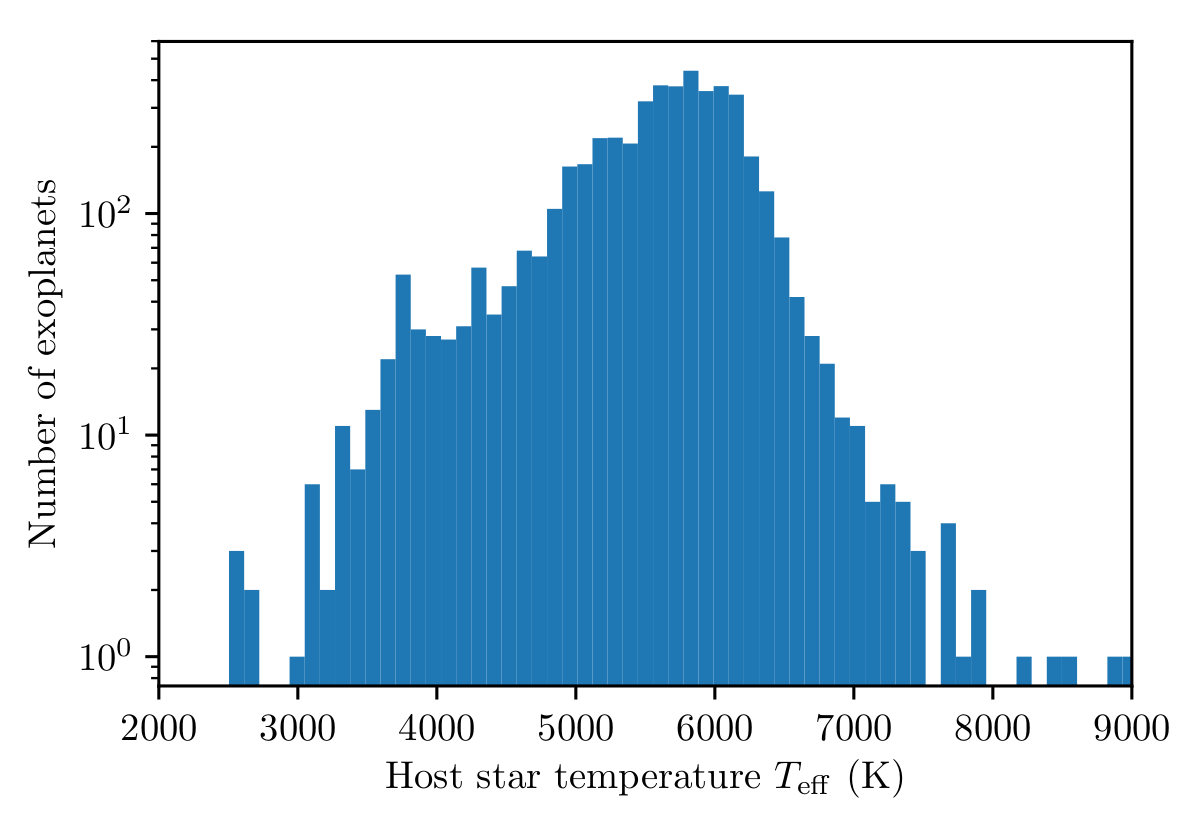
\includegraphics[width=\linewidth]{fig_histo_teff}

\includegraphics[width=\linewidth]{fig_histo_ld}
\caption{\label{fig:ld}Top: Linear LD as a function of $T_{\rm eff}$ for the TESS bandpass \citep{2017A&A...600A..30C} using log[M/H]=0, logg=4.5, Phoenix model type R/pc/LSQ. The range remains the same assuming other parameters or models. Middle: Histogram for the number of transiting exoplanets as a function of $T_{\rm eff}$ from \url{exoplanets.org} \citep{2014PASP..126..827H}. Bottom: Resulting histogram for the number of transiting exoplanets as a function of linear LD using the function shown on top.}
\end{figure}

\clearpage

\begin{figure}
\includegraphics[width=\linewidth]{fig_earth_lds_long_wavelengths}
\caption{\label{fig:wavelength}Simulated transit light curves of the Earth transiting the Sun across its entire diameter using LD data from \citet{1998A&A...333..338H}. Transit light curves for different wavelengths from the UV (300\,nm) to the NIR ($2.4\,\mu$m) are increasingly box-shaped. \RH{K{\"o}nnen wir Kurven f{\"u}r kurze Wellenl{\"a}ngen blau malen und f{\"u}r lange Wellenl{\"a}ngen rot -- und dann dazu eine Legende?}}
\end{figure}


\software{
Astropy \citep{2018AJ....156..123A}, NumPy \citep{numpy:2011}, SciPy \citep{scipy:2001}, Matplotlib \citep{matplotlib:2007}}

\bibliography{references}
\end{document}
